\section{Message Ownership in SOS}
\label{sec:example}

We illustrate our technique for static checking of dynamic
resources through an example of dynamic memory
management in SOS~\cite{sos}.
The SOS kernel supports dynamic linking of modules and has a dynamic memory
subsystem that can be used by the modules to create and pass around messages
as well as to store dynamically created state.
While providing a great deal of flexibility and expressiveness to
programmers, these abilities also
introduce programmer obligations to correctly access and manage memory.
Since the underlying hardware
does not have memory protection, following a dangling pointer
may cause the entire system to crash.
Since SOS runs on highly memory-constrained hardware, memory leaks can
bring down the system very quickly.
%We illustrate the ownership model of resource usage applied 
%to memory management in SOS.

\begin{figure}[t]
\centering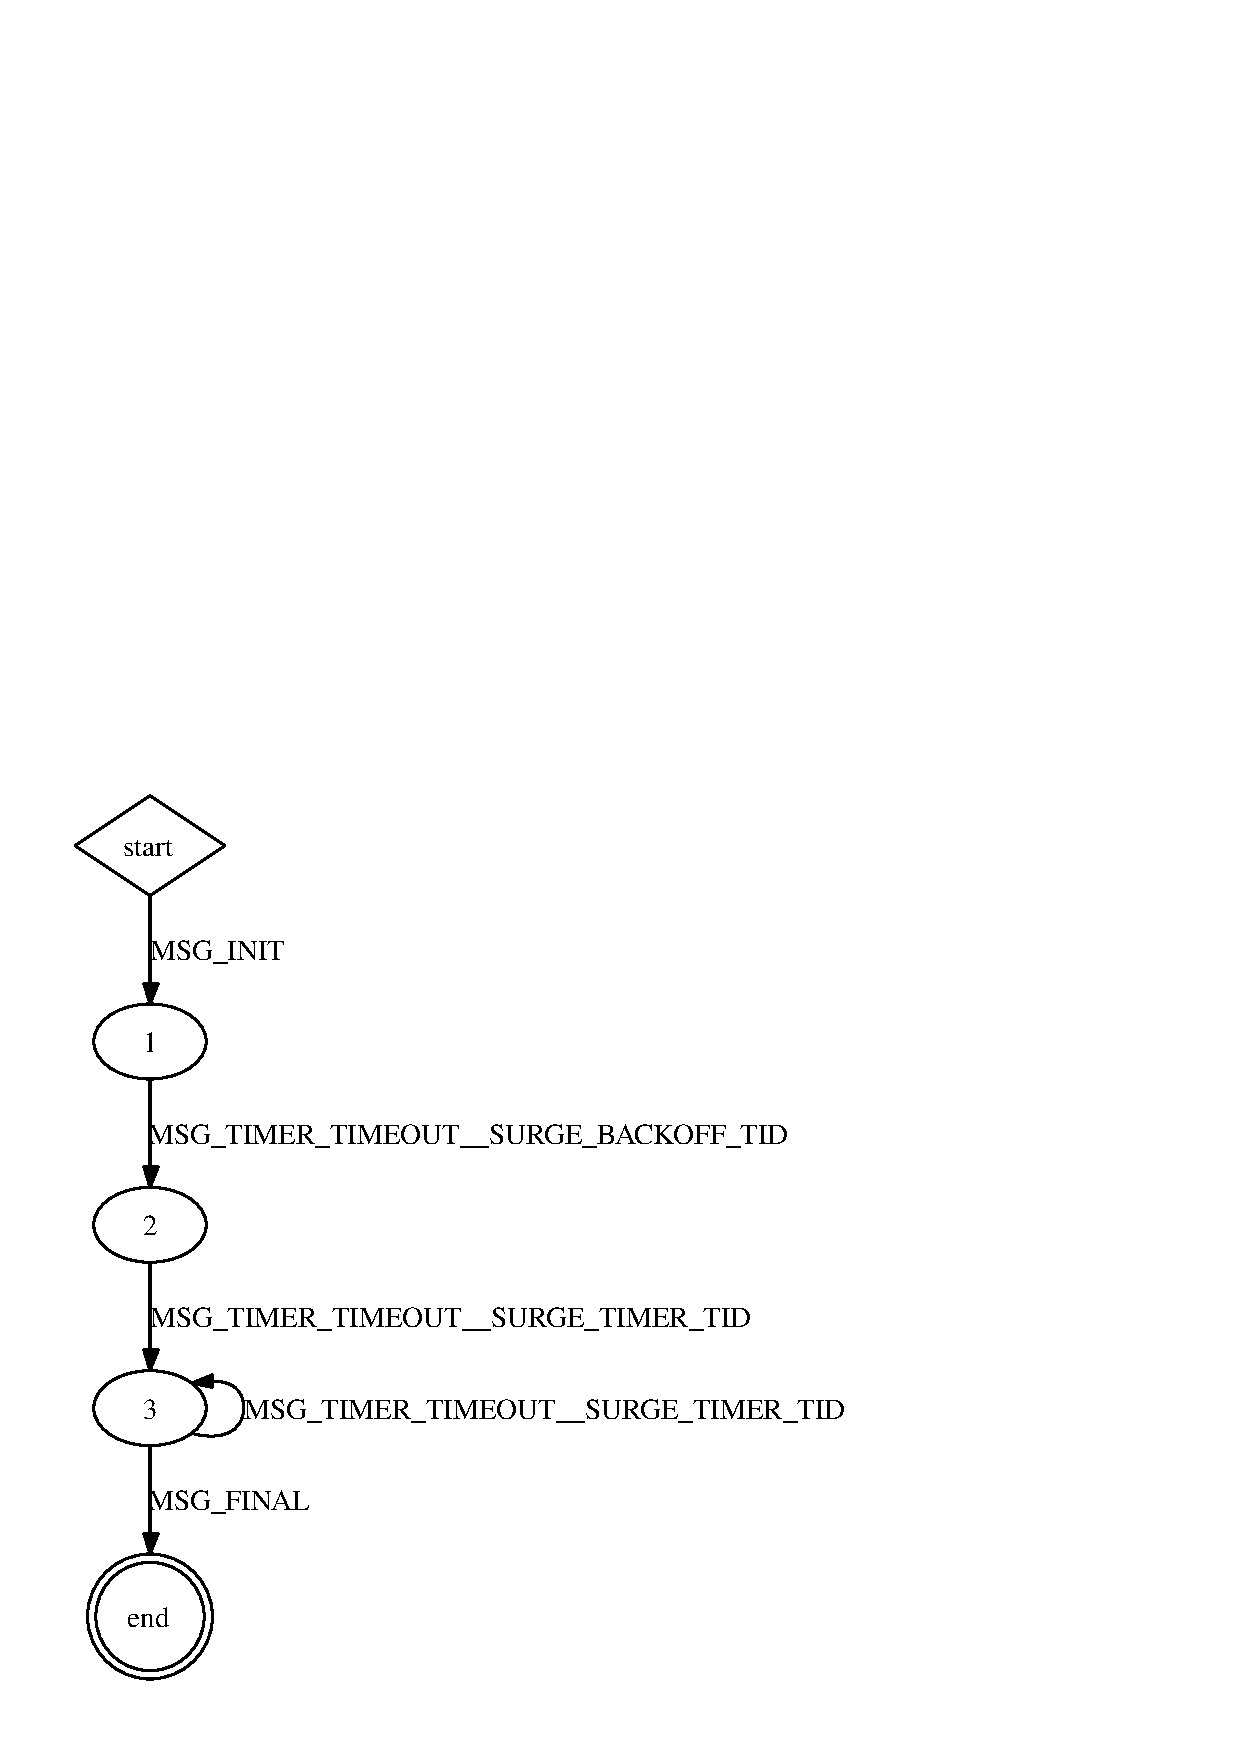
\includegraphics[angle=270,width=4.1in]{surge}
\caption{{\tt surge} dataflow\label{fig:surge-dataflow}}
\end{figure}


\begin{figure}[t]
\input{surge.c}
\caption{SOS implementation of {\tt surge}\label{fig:surge}}
\end{figure}

\subsection{{\tt surge}}

Figure~\ref{fig:surge} shows a portion of the 
SOS module that implements {\tt surge},
a simple sensor network application
that takes sensor readings and sends the readings over a multihop network
to a base station~\cite{nesC}. 
The function
{\tt surge\_module} is the entry point into {\tt surge}
for messages from the kernel and from other
modules. 
The function takes two arguments: a pointer to
the module's persistent state, which
is saved in the kernel, and a pointer to the current message.
The code for the function is a {\tt switch}
statement that appropriately handles each kind of message. 
%Certain messages have predefined meanings in SOS, for example, the message
%{\tt MSG\_INIT} initializes the module state (and is guaranteed to be sent
%by the kernel before any other messages), and the message {\tt MSG\_FINAL}
%cleans up the module before it is removed by the kernel.
Figure~\ref{fig:surge} shows the handlers for the messages
{\tt MSG\_DATA\_READY} and {\tt MSG\_TR\_DATA\_PKT}.

A sensor sends the message {\tt MSG\_DATA\_READY} to the surge module
when requested sensor data is ready to be read. The sensor data
is passed as the {\tt data} field of the message, which in general
always contains a message's payload.  Upon receiving this message,
the {\tt surge} message handler
allocates a new packet ({\tt ker\_malloc})
to be sent to the base station and posts a message ({\tt post\_long})
to the tree-routing module in order to forward the sensor data.  The
{\tt post\_long} call is asynchronous, causing the kernel to 
package up all the given arguments into a {\tt
  Message} structure and to schedule this message for eventual delivery.

The message {\tt MSG\_TR\_DATA\_PKT} is sent by the tree-routing module
when data is received at the base station node.
Upon receiving this message, the {\tt surge} message handler 
confirms that 
the current node is the base station.  If so, 
the message handler 
forwards the data to the UART driver via an
asynchronous message send ({\tt post\_net}).

%% In each case, the data is handled using an ownership principle: data is 
%% accessed only when it has been claimed via {\tt ker\_msg\_take\_data}
%% (or allocated in the current module),
%% and never accessed again once it has been released to other modules.

\subsection{Dynamic Memory Management in SOS}

The SOS kernel provides an API for programmers to manage
dynamic memory.  As shown in Figure~\ref{fig:surge}, the
{\tt ker\_malloc} function acts as expected, allocating a new block of
memory.  The kernel also provides a {\tt ker\_free} function for
destroying dynamically allocated memory.

In order to provide a simple form of automatic
garbage collection for dynamically allocated memory, the SOS kernel
imposes an {\em ownership}
model on dynamic memory~\cite{sos}.  Each block of memory
has a unique owner at any point in time, and the kernel maintains a mapping
from each block of memory to its owner.  A block's initial owner is
the module that allocates that block.  For example,
the call to {\tt ker\_malloc} sets the {\tt surge}
module as the initial owner of the newly allocated block.
When a module is removed from the system at run time, the
kernel automatically frees all memory owned by that module.

%% The memory ownership model used in SOS requires data to have exactly one well
%% defined owner at all times.
%% %
%% All memory blocks are originally owned by the kernel.
%% %
%% Modules can allocate memory from the kernel and release allocated memory back
%% to the kernel's control.
%% %
%% Modules can also transfer ownership of memory blocks to other modules.


%% A module can gain ownership of a block of memory by calling
%% \texttt{ker\_malloc} to allocate a block from the kernel. 
%% %
%% A successful call to \texttt{ker\_malloc} gives the calling module ownership
%% of the returned block.
%
%% A module can also gain ownership of a block by calling
%% \texttt{ker\_msg\_take\_data} on an incoming message.
%% %
%% This causes the module to either: claim ownership of the data payload if the
%% payload was released by the sender of the message, or gain ownership of a new
%% copy of the data payload if the sender of the message did not release the
%% data.
%% %
%% Both \texttt{ker\_malloc} and \texttt{ker\_msg\_take\_data} can return a NULL
%% pointer, signaling that the allocation attempt failed.
%% %
%% Finally, a module gains ownership of a block of memory by calling a
%% function with a formal parameter that has the \texttt{sos\_claim} attribute
%% set.

The SOS kernel provides facilities for ownership transfer.  Such
transfer occurs in two phases.  
%
First, the owner of a block of dynamically allocated memory can explicitly {\em
  release} ownership of that block when it is passed as the payload in
  a message.  This is accomplished by setting the
\texttt{SOS\_MSG\_RELEASE} flag in the corresponding
  {\tt post\_*} call.  
  For example, the {\tt surge}
  module releases ownership of the newly allocated {\tt pkt} upon
  sending it to the tree-routing module.
  Second, a module can acquire ownership of a message's payload, which
  is stored in the {\tt data} field, by calling
\texttt{ker\_msg\_take\_data} on an incoming message.  The function
  returns a pointer to the message's payload.  For example,
  if the current node is the base station,
  the {\tt surge} module explicitly takes ownership of the given
  message's data under the name {\tt payload}.

%
There are four release/take scenarios to consider.  If data is
both released by its sender and taken by its receiver, then ownership
of the data is transferred from the sender to the receiver.
If data is released by its sender but not taken by its receiver,
then the kernel automatically frees the memory after
the receiver's message handler completes.  If data is not released
by its sender but is taken by its receiver, then the sender keeps
ownership of the original message and the receiver gains ownership of
a new block of memory containing a copy of that data.  Finally, if the data is
not released by the sender and not claimed by the receiver, then the sender
keeps ownership of the original message and the receiver has direct access to
``borrowed'' data for a limited period of time.  This last case is not generally used
in SOS due to the synchronization complications that can result.
%% Rather, sharing
%% of this type is accomplished through direct (synchronous) function calls
%% in which the scope of the ``borrowed'' data is limited to the duration of the
%% function call.
%
%% Both \texttt{ker\_malloc} and \texttt{ker\_msg\_take\_data} can return a NULL
%% pointer, signaling that the allocation attempt failed.
%% %
%% Finally, a module gains ownership of a block of memory by calling a
%% function with a formal parameter that has the \texttt{sos\_claim} attribute
%% set.


%
%% Functions that can use this flag are: \texttt{post}, \texttt{post\_net} and
%% \texttt{post\_long}.
%% %
%% This causes the ownership of the data to be transfered to kernel.
%% %
%% The kernel then gives ownership to the receiver of the message if the
%% receiver requests ownership of the data, or returns the data block back to the
%% free pool for memory allocation if the receiver is not present or if the
%% receiver does not request ownership of the data.
%% %
%% Second, a data block can be passed to another module by having the owner of
%% the data call the function \texttt{ker\_change\_own} and supplying the module
%% ID of the receiving module.
%% %
%% Third, a data block can be passed to another module via a call to a function
%% that directly or transitively releases the block to another module. 
%% %
%% In this case the prototype of the function call should add the attribute
%% \texttt{sos\_release} to the formal parameter of the data released by the
%% function.
%% %
%% Note that the first case listed above is simply a common special case of this
%% third rule.
%% %
%% In some situations a function may conditionally release data.
%% %
%% This is currently facilitated by using the \texttt{sos\_may\_release}
%% attribute in conjunction with a flag describing if the data is to be released,
%% as is the case with the messaging API.


%% A module should only release data that it owns.
%% %
%% Released data is considered dead to the module that releases it and should
%% not be referenced.
%% %
%% The module that receives the released data becomes the new owner of the block
%% with all the responsibilities associated with block ownership.


%% Modules are responsible for deallocating, releasing, or storing a persistent
%% reference to blocks that they own.
%% %
%% A block can be deallocated with a call to \texttt{ker\_free} and should only
%% be deallocated by the module that owns the block.  
%% %
%% Releasing data is described above.
%% %
%% A persistent reference to data is be created by storing a reference to the
%% data in a module's state.


%% After a block becomes dead to a module, it may not be accessed in any form by
%% the previous owner.
%% %
%% Program statements that follow the statement that killed that data my not
%% dereference the data in any form.
%% %
%% Program statements that came before the statement that killed the data should
%% not deallocate, release, or create a persistent reference to the freed data.

%%%%%%%%%%%%%%%%%%%%%%%%%%%%%%%%%%%%%%%%%%%%%%%%%%%%%%%%%%%%

\subsection{Static Ownership Checking}

SOS's original concept of ownership as described above
provides a simple form of
garbage collection at run time.
While this can help
reduce the complexity of managing
dynamic memory, it is not sufficient to
prevent memory errors such as dangling pointers and memory leaks.
For example, nothing prevents a module from freeing some memory while
another module (or even the same module) still has a pointer to that
memory.  If that pointer is ever accessed later, an invalid dereference
will result.  Further, garbage collection introduces the potential for
more dangling pointer errors, since the removal of a module implicitly
frees the memory it owns, even if other modules have pointers to that
memory.

%% The basic problem is that SOS's intuitive concept of ownership is
%% not enforced.  There is no guarantee that
%% a program's ownership directives and
%% annotations are consistent with the rest of the program.  Further,
%% there is no explicit notion of what it means to be consistent, namely the
%% rights and responsibilities of owners and non-owners with respect to
%% dynamic memory.  Instead, the burden is on the programmer to ensure
%% that the implicit ownership protocol is properly respected.

In this work, we augment SOS's ownership directives to
provide a protocol governing
memory management that is sufficient to ensure the absence of
memory errors.
Our protocol makes explicit a common programming idiom in
sensor-network systems, whereby data is rarely shared but instead
follows a producer/consumer model.
We have built a tool that checks for violations of this protocol on
each SOS module at compile time.

Informally, the rules of the protocol can be stated as
follows:
\begin{itemize}

\item A module may only manipulate the memory that it owns.

\item A module that takes ownership of a block of memory (either
  through {\tt ker\_malloc} or {\tt ker\_msg\_take\_data}) must either
  free that memory, release it, or store it in the module's
  persistent state.

\item A module may only free or release memory that it owns.  After a module
  frees or releases memory, it may not access or update that memory.
\end{itemize}
Because only the owner can manipulate or free its
memory, dangling pointers are avoided.  Because all memory must be
either freed, released or persistently stored by its owner,
memory leaks are avoided.


\subsection{{\tt surge} Revisited}

Our tool is able to validate at compile time that the
{\tt surge} module properly obeys the ownership protocol.
The {\tt MSG\_DATA\_RDY} message handler
allocates {\tt pkt} and takes
ownership. This pointer is then dereferenced in order to provide the
sensor data
to be sent up the routing tree.
This pointer manipulation is safe since the module has ownership.
The module then
releases ownership by posting {\tt pkt} to the tree routing module
using the {\tt SOS\_MSG\_RELEASE} tag.  After this release, the
module does not access
{\tt pkt} again and does not store it, ensuring that access to the
pointer is indeed released. 

The handler for {\tt MSG\_TR\_DATA\_PKT} also conforms to the
protocol.   When the current
node is the base station, the handler explicitly acquires ownership of
the message's data
using {\tt ker\_msg\_take\_data}.  This allows the module to
manipulate the data and to pass it to
the UART.  The {\tt post\_net} call
explicitly releases the data, fulfilling the module's obligation to
that data.   After the release, the data
is no longer accessed or stored.

While the {\tt surge} code is correct, small changes to the code can
easily cause problems to occur at run time, and our static checker
catches these potential errors.  For example, suppose the handler for
{\tt MSG\_DATA\_READY} did not release ownership of {\tt pkt} by setting the 
{\tt SOS\_MSG\_RELEASE} flag in the call to {\tt post\_long}.
In that case, the module would leak the memory allocated for {\tt pkt}.
Indeed, our checker flags this
modified version of the code as erroneous, since {\tt surge} would not be
freeing, releasing, or storing the data for which it has taken ownership.

\subsection{Function Attributes}

%% The next section details the way in which our tool conservatively
%% ensures at compile time that SOS modules obey this protocol.  The
%% heart of the checker is a suite of dataflow analyses that statically
%% approximate the dynamic ownership relationships.  
%% So far, we have described the analysis for the {\em intra-procedural case},
%% i.e., when there are no function calls.
Our analysis is {\em modular}:  
each function in a module is analyzed in isolation.  To make checking
of a function body precise in the presence of calls to other
functions, we employ
{\em ownership attributes} for function headers that capture the memory-related
behavior of a called function.
We add two attributes to the SOS API: {\tt sos\_claim} and {\tt sos\_release}.
A formal parameter or return value
that has the {\tt sos\_claim} attribute indicates that the
caller must take ownership of the associated memory after a call.
This annotation, for example, would be used to annotate a function that
wraps a call to {\tt ker\_malloc}, allowing that function's callers to
be properly checked without access to the function's implementation.
Similarly, an {\tt sos\_release} attribute on a formal parameter
%
indicates that ownership of the parameter is transferred from the caller of the
function to the callee.
%indicates that the parameter's contents are either released or freed
%(directly or indirectly) by the function.
%
If a parameter does not have an ownership attribute, memory ownership
is unchanged.
%% Our tool makes use of ownership attributes to precisely check callers
%% of a function.  
Our tool ensures that these attributes are employed wherever 
necessary, when checking the implementation of each function. 
%
%% Attributes do not need to reside in the code.  An annotation configuration
%% file can be used by the checker to insert attributes during analyses.  The
%% annotations in this configuration look like:
%% %
%% \begin{footnotesize}
%% \begin{verbatim}
%% add annotations "ker_malloc" [Some "sos_claim"; None; None];
%% \end{verbatim}
%% \end{footnotesize}
%% %
%% specifying that the {\tt sos\_claim} attribute should be added to the 
%% data returned by {\tt ker\_malloc} and that the two formal parameters need
%% no additional ownership attributes.  Our tool assumes that functions not described in
%% the annotation configuration need no other attributes added to them.  
In practice, we have found that a small set of annotations
is sufficient for precise analysis.
%% to obviate the need for explicit attributes annotations in user code.

\subsection{Generality}

Memory errors in SOS were the original motivation for our work.
Further, the existing ownership directives for dynamic
memory in SOS facilitated the creation of our tool.  However, we stress that
the underlying protocol that we enforce
is completely independent of both SOS and of
memory in particular.  For example, it would be straightforward to
apply our tool to track resources other than memory in SOS, and
we could similarly port our tool to enforce an ownership protocol on
nesC's static buffers rather than
SOS's dynamic memory.

